%
%  PARA TRABALLOS EN GALLEGO USAR (LINEA 12): \usepackage[galician]{babel}
%  PARA TRABALLOS EN CASTELLANO USAR (LINEA 13): \usepackage[spanish]{babel}
%
% Para los acentos usamos codificacion UTF-8 (LINEA 10): \usepackage[utf8]{inputenc} 
% Si se usase la codificacion es_ES.ISO-8859-1 (LINEA 11): \usepackage[latin1]{inputenc}
% La conversion de acentos se hace con: iconv -f UTF-8 -t ISO-8859-1 filename.tex
%
% Como se incluyen figuras eps hay que compilar con: latex traballo , dvipdf traballo
%

\documentclass[12pt,twoside,a4paper]{book}
% pódense engadir todos os packages necesarios
\usepackage[utf8]{inputenc}
% \usepackage[latin1]{inputenc}
\usepackage[galician]{babel}
% \usepackage[spanish]{babel}
\usepackage{graphicx}
\usepackage[dvips]{epsfig}
\usepackage{amssymb}
\usepackage{eurosym}
\usepackage{float}
\usepackage{latexsym}
\usepackage{a4}
\usepackage{listings}
% \usepackage{hyperref} % menús no pdf pero non leva ben co package galician


\addto\captionsgalician{\def\contentsname{Memoria tipo B -- \'{I}ndice xeral }}
	

\begin{document}
\pagestyle{empty}
\begin{center}
	{\bf\Large UNIVERSIDADE DE SANTIAGO DE COMPOSTELA}
	
	\vspace{0.5cm}
	
\includegraphics[width=5cm]{figuras/logo_usc.eps}
	
	\vspace{0.5cm}
	{\bf\large ESCOLA TÉCNICA SUPERIOR DE ENXEÑARÍA}
	
	\vspace{3cm}
	{\bf\LARGE Herramienta para la creación y edición colaborativa de documentos}
	
	%\vspace{0.5cm}
	%{\bf\LARGE Subtítulo do Traballo de Fin de Grao}
\end{center}

\vspace{2cm}
\hspace{4cm}\begin{tabular}{l}
	{\it\Large Autor:} \\
	{\bf\Large Pablo Tarrío Otero} \\
	~ \\
	{\it\Large Tutores:} \\
	{\bf\Large Manuel Lama Penín} \\
	{\bf\Large Juan Carlos Vidal Aguiar} \\
	{\bf\Large Víctor José Gallego Fontenla} \\
\end{tabular}

\vspace{2cm}
\begin{center}
	{\bf\Large Grado en Ingeniería Informática}
	
	\vspace{0.5cm}
	{\bf\large Julio 2022}
	
	\vspace{0.5cm}
	Trabajo de Fin de Grado presentado en la {\it Escola Técnica Superior de Enxeñaría} de la {\it Universidade de Santiago de Compostela} para la obtención del Grado en Ingeniería Informática
\end{center}
\cleardoublepage
\pagestyle{plain}
\pagenumbering{roman}

\includegraphics[width=4cm]{figuras/logo_usc.eps}

\vspace{1cm}
{\bf D. (Nome da titora ou do titor)}, Profesor/a do Departamento de Electrónica e Computación da Universidade de Santiago de Compostela, e {\bf D. (Nome da cotirora ou do cotitor)}, Profesor/a do Departamento de Electrónica e Computación da Universidade de Santiago de Compostela,

\vspace{1cm}
INFORMAN:

\vspace{1cm}
Que a presente memoria, titulada {\it (Título do traballo)}, presentada por {\bf D. (Nome da autora ou do autor do traballo)} para superar os créditos correspondentes ao Traballo de Fin de Grao da titulación de Grao en Enxeñaría Informática, realizouse baixo nosa titoría no Departamento de Electrónica e Computación da Universidade de Santiago de Compostela.

\vspace{1cm}
E para que así conste aos efectos oportunos, expiden o presente informe en Santiago de Compostela, a (Data):

\vspace{2cm}
\begin{tabular}{lll}
	Titor/a, & Cotitor/a, & Alumno/a, \\
	~ \\
	~ \\
	~ \\
	~ \\
	~ \\
	~ \\
	~ \\
	(Nome do titor/a) & (Nome do cotitor/a) & (Nome do alumn/a)
\end{tabular}

 % paxina de certificación (optativa)
\cleardoublepage
\pagestyle{plain}
\chapter*{Agradecementos}
Se se quere pór algún agradecemento, este vai aquí.

 % paxina de agradecementos (optativa) 
\cleardoublepage
\pagestyle{plain}
\chapter*{Resumo}
Breve resumo das principais contribucións do traballo.

 % páxina de resumo (optativa) 

\cleardoublepage
\pagestyle{plain}
\tableofcontents
\listoffigures
\listoftables

% Agora incluimos os capítulos. Cambiamos a numeración e as cabeceiras
\cleardoublepage
\pagenumbering{arabic}
\setcounter{page}{1}
\pagestyle{headings}
\chapter{Introdución}
\hyphenation{In-te-re-se}

Obxectivos Xerais, Relación da Documentación que conforma a Memoria, Descrición do Sistema, Información Adicional de Interese (métodos, técnicas ou arquitecturas utilizadas, xustificación da súa elección, etc.).

\cleardoublepage
\chapter{Especificación de Requisitos}

Especificación dos requisitos máis relevantes do Sistema, xunto coa información que este debe almacenar e as interfaces con outros Sistemas, sexan hardware ou software, e outros requisitos (rendemento, seguridade, etc.).

\cleardoublepage
\chapter{Deseño}

Debe describirse como se realiza o Sistema, a división deste en diferentes compoñentes e a comunicación entre eles. Así mesmo, determinarase o equipamento hardware e software necesario, xustificando a súa elección no caso de que non fose un requisito previo. Debe achegarse a un nivel suficiente de detalle que permita comprender a totalidade da estrutura do produto desenvolvido, utilizando no posible representacións gráficas.
\cleardoublepage
\chapter{Probas}

Plan de probas (con evidencias) que verifica a funcionalidade e correctitude global do sistema, e se leva a cabo.
\cleardoublepage
\chapter{Exemplos (eliminar capítulo na versión final)}

\section{Un exemplo de sección}
Esta é {\it letra cursiva}, esta é {\bf letra negrilla}, esta é \underline{letra subrallada}, e esta é {\tt letra curier}. Letra {\tiny tiny}, {\scriptsize scriptsize}, {\small small}, {\large large}, {\Large Large}, {\LARGE LARGE} e moitas más. Exemplo de fórmula: $a=\int_o^\infty f(t)dt$.  E agora unha ecuación aparte:

\begin{equation}
S=\sum_{i=0}^{N-1} a_i^2 .
\label{mi_ecuacion}
\end{equation}

As ecuaciones se poden referenciar: ecuación (\ref{mi_ecuacion}).

\subsection{Un exemplo de subsección}
O texto vai aquí.
\subsection{Otro exemplo de subsección}
O texto vai aquí.
\subsubsection{Un exemplo de subsubsección}
O texto vai aquí.
\subsubsection{Un exemplo de subsubsección}
O texto vai aquí.
\subsubsection{Un exemplo de subsubsección}
O texto vai aquí.
\section{Exemplos de figuras e cadros}

A figura número \ref{enlace1}.

O cadro (taboa) número \ref{enlace2}.

\begin{figure}
\centerline{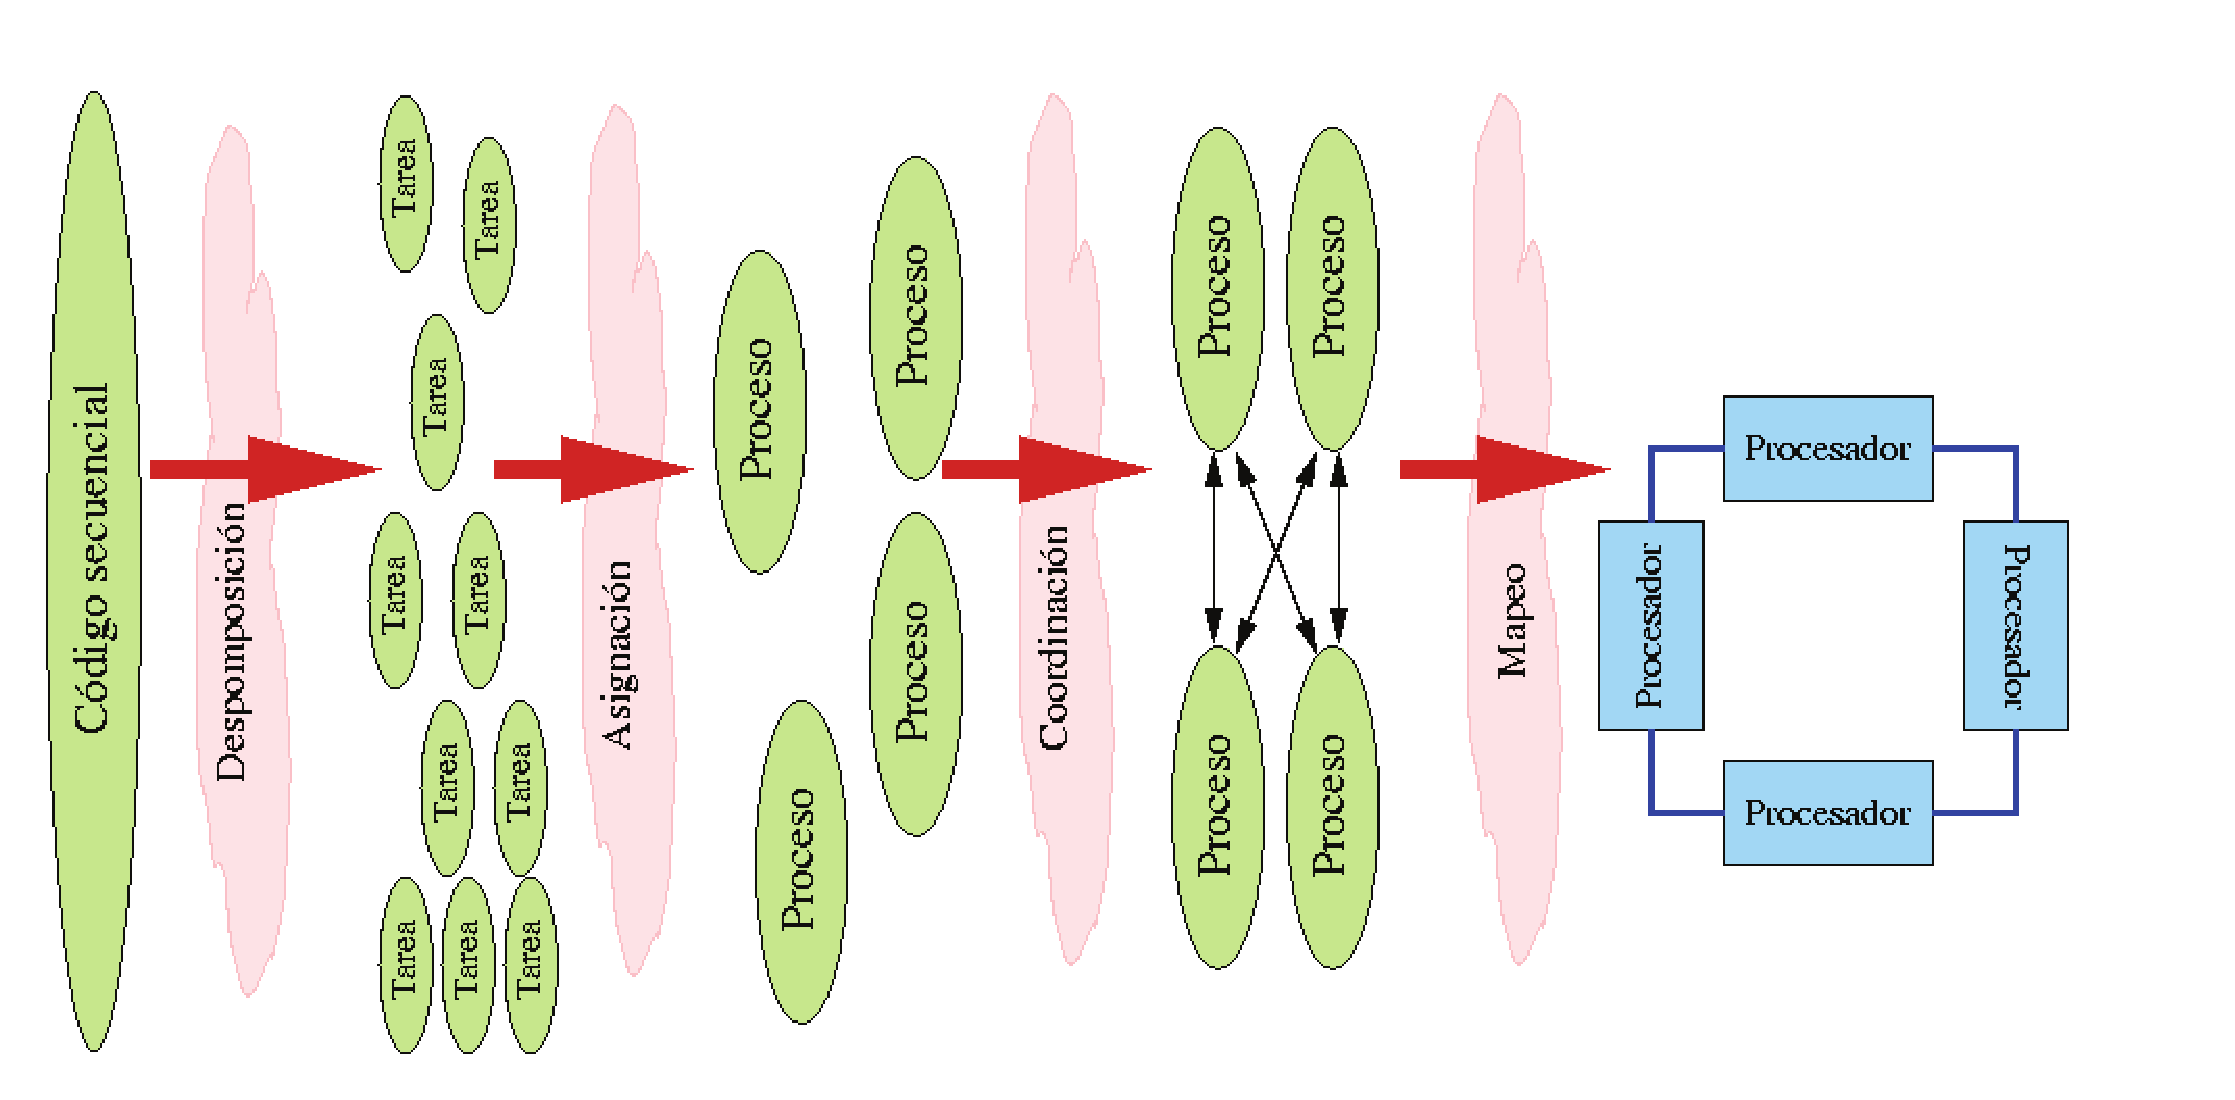
\includegraphics[width=15cm]{figuras/figura01.eps}}
\caption{Esta é a figura de tal e cal.}
\label{enlace1}
\end{figure}

\begin{table}
\begin{center}
\begin{tabular}{|l||r|c|} \hline
Izquierda & Derecha & Centrado  \\ \hline\hline
ll & r & cccc \\ \hline
llll & rrr & c \\ \hline
\end{tabular}
\caption{Esta é a táboa de tal e cal.}
\label{enlace2}
\end{center}
\end{table}

\section{Exemplos de referencias á bibliografía}
Este é un exemplo de referencia a un documento descargado da web \cite{cuda}. E este é un exemplo de referencia a unha páxina da wikipedia \cite{cdma}. Agora un libro \cite{gonzalez} e agora unha referencia a un artigo dunha revista \cite{patricia}. Tamén se poden pór varias referencias á vez \cite{cuda,gonzalez}.

\section{Exemplos de enumeracións}

Con puntos:

\begin{itemize}
\item Un.
\item Dous.
\item Tres.
\end{itemize}

Con números:

\begin{enumerate}
\item Catro.
\item Cinco.
\item Seis.
\end{enumerate}

Exemplo de texto verbatim:

\begin{verbatim}
O texto        verbatim 
     se visualiza tal
            como se escribe
\end{verbatim}

Exemplo de código C:

\lstset{language=C}

\begin{lstlisting}
#include <math.h>
main()
{  int i, j, a[10];
   for(i=0;i<=10;i++) a[i]=i; // comentario 1
   if(a[1]==0) j=1; /* comentario 2 */
   else j=2;
}
\end{lstlisting}

Exemplo de código Java:

\lstset{language=java}

\begin{lstlisting}
class HelloWorldApp {
    public static void main(String[] args) {
        System.out.println("Hello World!"); // Display the string.
    }
}
\end{lstlisting}



%
% Engadir os capitulos que fagan falta
%
\cleardoublepage
\chapter{Conclusións e posibles ampliacións}

O traballo describe o grao de cumprimento dos obxectivos. Posibles vías de mellora.


% Aquí empezan os apéndices
\appendix
\cleardoublepage
\chapter{Manuais técnicos}

En función do tipo de Traballo e metodoloxía empregada, o contido poderase dividir en varios documentos. En todo caso, neles incluirase toda a información precisa para aquelas persoas que se vaian encargar do desenvolvemento e/ou modificación do Sistema (por exemplo código fonte, recursos necesarios, operacións necesarias para modificacións e probas, posibles problemas, etc.). O código fonte poderase entregar en soporte informático en formatos PDF ou postscript.
\cleardoublepage
\chapter{Manuais de usuario}

Incluirán toda a información precisa para aquelas persoas que utilicen o Sistema: instalación, utilización, configuración, mensaxes de erro, etc. A documentación do usuario debe ser autocontida, é dicir, para o seu entendemento o usuario final non debe precisar da lectura doutro manual técnico.

\cleardoublepage
\chapter{Licenza}
Se se quere pór unha licenza (GNU GPL, Creative Commons, etc), o texto da licenza vai aquí.


\cleardoublepage
\markboth{BIBLIOGRAFÍA}{BIBLIOGRAFÍA}
\addcontentsline{toc}{chapter}{Bibliografía}


\begin{thebibliography}{99}
% EXEMPLO DE DOCUMENTO DESCARGADO DA WEB
\bibitem{cuda} Nvidia CUDA programming guide. Versión 2.0, 2010. Dispoñible en {\it http://www.nvidia.com}.

% EXEMPLO DE PÁXINA DA WIKIPEDIA
\bibitem{cdma} Acceso múltiple por división de código. Artigo da wikipedia ({\it http://es.wikipedia.org}). Consultado o 2 de xaneiro do 2010.

% EXEMEPLO DE LIBRO
\bibitem{gonzalez} R.C. Gonzalez e R.E. Woods, {\it Digital image processing}, 3ª edición, Prentice Hall, New York, 2007.

% EXEMPLO DE ARTIGO DE REVISTA
\bibitem{patricia} P. González, J.C. Cartex e T.F. Pelas, ``Parallel computation of wavelet transforms using the lifting scheme'', {\it Journal of Supercomputing}, vol. 18, no. 4, pp. 141-152, junio 2001.
\end{thebibliography}



\end{document}
